\let\negmedspace\undefined
\let\negthickspace\undefined
\documentclass[journal]{IEEEtran}
\usepackage[a5paper, margin=10mm, onecolumn]{geometry}
\usepackage{lmodern} % Ensure lmodern is loaded for pdflatex
\usepackage{tfrupee} % Include tfrupee package
\usepackage[utf8]{inputenc}
\usepackage[T1]{fontenc}

\setlength{\headheight}{1cm} % Set the height of the header box
\setlength{\headsep}{0mm}     % Set the distance between the header box and the top of the text

\usepackage{gvv-book}
\usepackage{gvv}
\usepackage{cite}
\usepackage{amsmath,amssymb,amsfonts,amsthm}
\usepackage{algorithmic}
\usepackage{graphicx}
\usepackage{textcomp}
\usepackage{xcolor}
\usepackage{txfonts}
\usepackage{listings}
\usepackage{enumitem}
\usepackage{mathtools}
\usepackage{gensymb}
\usepackage{comment}
\usepackage[breaklinks=true]{hyperref}
\usepackage{tkz-euclide} 
\usepackage{listings}
\usepackage{gvv}                                        
\def\inputGnumericTable{}                                 
%\usepackage[latin1]{inputenc}
\usepackage{color}                                            
\usepackage{array}                                            
\usepackage{longtable}                                       
\usepackage{calc}                                             
\usepackage{multirow}                                         
\usepackage{hhline}                                           
\usepackage{ifthen}                                           
\usepackage{lscape}

\begin{document}
\bibliographystyle{IEEEtran}
\vspace{3cm}

\title{1.1.5.15}
\author{EE24BTECH11045 - N.Tapasvi}
{\let\newpage\relax\maketitle}
Question:\\
The midpoint of the line segment joining $\vec{A}\myvec{2a\\4}$ and $\vec{B}\myvec{\text{-}2\\3b}$ is $\vec{M}\myvec{1\\2a+1}$. Find the values of a and b.
\hfill (10,2019)

\solution
\begin{table}[h!]    
  \centering
  \begin{tabular}[12pt]{ |c| c|}
    \hline
    \textbf{Variable} & \textbf{Description}\\ 
    \hline
	$\vec{A}$ & $\myvec{2a\\4}$\\
	\hline
	$\vec{B}$ & $\myvec{-2\\3b}$\\
	\hline
	$\vec{C(Midpoint)}$ & $\myvec{1\\2a+1}$\\
	\hline
	$\vec{a,b}$ & Values to be found\\
\end{tabular}

  \caption{Variables Used}
  \label{tab1-1.5-15}
\end{table}\\


The section formula in general:

\[
\begin{pmatrix}
x_M \\
y_M
\end{pmatrix}
=
\frac{1}{m + n}
\begin{pmatrix}
m x_2 + n x_1 \\
m y_2 + n y_1
\end{pmatrix}
\]

Since the midpoint divides the segment in the ratio 1:1,\( m = n = 1 \):

\[
\begin{pmatrix}
x_M \\
y_M
\end{pmatrix}
=
\frac{1}{2}
\begin{pmatrix}
x_2 + x_1 \\
y_2 + y_1
\end{pmatrix}
\]

Substitute the coordinates of points A and B:

\[
\begin{pmatrix}
x_M \\
y_M
\end{pmatrix}
=
\frac{1}{2}
\begin{pmatrix}
-2 + 2a \\
3b + 4
\end{pmatrix}
\]

Given midpoint \( M \) has coordinates \( (1, 2a + 1) \), so we can equate the coordinates:

For the \( x \)-coordinate:

\[
\frac{1}{2} (-2 + 2a) = 1 \quad \Rightarrow \quad -2 + 2a = 2 \quad \Rightarrow \quad 2a = 4 \quad \Rightarrow \quad a = 2
\]

For the \( y \)-coordinate:

\[
\frac{1}{2} (3b + 4) = 2a + 1 \quad \Rightarrow \quad \frac{1}{2} (3b + 4) = 2(2) + 1 \quad \Rightarrow \quad \frac{1}{2} (3b + 4) = 5
\]

Multiply both sides by 2:

\[
3b + 4 = 10 \quad \Rightarrow \quad 3b = 6 \quad \Rightarrow \quad b = 2
\]


Therefore, the values of \( a \) and \( b \) are:

\[
a = 2, \quad b = 2
\]
\begin{figure}[h!]
   \centering
	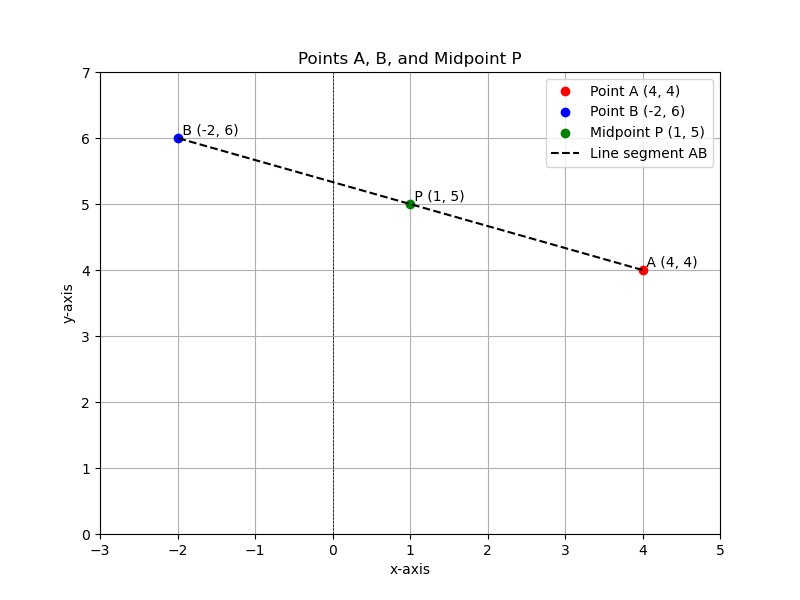
\includegraphics[width=1.15\linewidth]{/home/namala-tapasvi/Figure_1.png}
   \caption{Plot of the points A,B,M}
   \label{stemplot}
\end{figure}

\end{document}

